\documentclass[11pt]{report}

\usepackage{amsmath}
\usepackage{amssymb}
\usepackage{amsfonts}
\usepackage{dsfont}
\usepackage{epsfig}
\usepackage{times}
\usepackage{multicol}
%\usepackage{mcode}

\usepackage{bm}

\usepackage{footnote}
\makesavenoteenv{tabular}

\usepackage{enumerate}
%\usepackage{enumitem}
\usepackage{pdfpages}
%\usepackage{hyperref}
\usepackage{calc}
\usepackage{verbatim}

\usepackage{geometry}
\usepackage{parskip}
\geometry{margin=0.25in}

\DeclareMathOperator{\Prob}{\mathbb{P}}
\DeclareMathOperator{\Exp}{\mathbb{E}}
\DeclareMathOperator{\Var}{\text{Var}}
\DeclareMathOperator*{\argmin}{\arg\min}
\DeclareMathOperator{\SSS}{\mathcal{S}}
\DeclareMathOperator{\argmax}{\arg\max}

\newcommand{\E}{\mathbb{E}}
\newcommand{\R}{\mathbb{R}}

\newcommand{\ind}{{\mathds{1}}}

\newcommand{\bs}{\boldsymbol}

\renewcommand{\P}{\mathbb{P}}
\newcommand{\teq}{\triangleq}
\newcommand{\tr}{{\text{\tiny T}}}
\newcommand{\abs}[1]{\left| #1 \right|}
\begin{document}
\begin{center}
	{\bf\large APMA 1740/2610 2025: Homework 4}
\end{center}
%\noindent{\bf\Large BE SURE TO CHANGE TO THE APPROPRIATE HW NUMBER}
\medskip


\begin{enumerate}[1.]

	%%%%%%%%%%%%%%%%%%%%%%%%%%
	%			Problem 
	%%%%%%%%%%%%%%%%%%%%%%%%%%

	\item {\bf A simple two-category classification problem.}
	      Let $Y\in\{1,2\}$ be a random variable with $\Prob(Y=1)=0.45$. Given $Y=y$, let $X$ be a N$(y,y^2)$ random variable (i.e., normal with mean $y$ and standard deviation $y$). Let $f(x)$ denote the pdf of $X$, and let $f_y(x)=f(x|Y=y)$ denote the conditional pdf of $X$ given that $Y=y$. Let $r_y(x)=\Prob(Y=y|X=x)$ denote the conditional probability that $Y=y$ given $X=x$, defined in the usual way with Bayes' rule.
	      \begin{enumerate}
		      \item Find expressions for $f(x)$, $f_1(x)$, and $f_2(x)$. Plot all 3 on the same graph for $x\in(-4,8)$.

		            \color{blue}
		            \begin{align*}
			            f_1(x) & = f(x \; | \; Y = 1)                                                                                                               \\
			                   & \sim \mathcal N(1, 1)                                                                                                              \\
			                   & = \frac{1}{\sqrt{2\pi}} \exp\left(-\frac{(x - 1)^2}{2}\right)                                                                      \\
			            f_2(x) & = f(x \; | \; Y = 2)                                                                                                               \\
			                   & = \sim \mathcal N(2, 4)                                                                                                            \\
			                   & = \frac{1}{2\sqrt{2\pi}} \exp\left(-\frac{(x - 2)^2}{8}\right)                                                                     \\
			            f(x)   & = 0.45 f_1(x) + 0.55 f_2(x)                                                                                                        \\
			                   & = \frac{0.45}{\sqrt{2\pi}} \exp\left(-\frac{(x - 1)^2}{2}\right) + \frac{0.55}{2\sqrt{2\pi}} \exp\left(-\frac{(x - 2)^2}{8}\right)
		            \end{align*}

		            \begin{center}
			            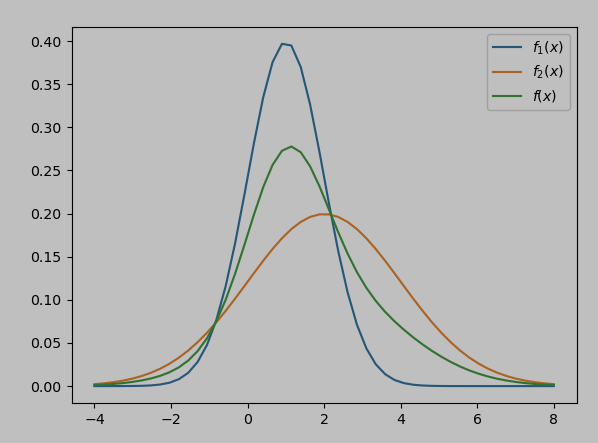
\includegraphics[width=0.8\textwidth]{Images/1a.png}
		            \end{center}
		            \color{black}

		      \item Find expressions for $r_1(x)$ and $r_2(x)$. Plot both on the same graph for $x\in(-4,8)$.

		            \color{blue}
		            \begin{align*}
			            r_1(x) & = \P(Y = 1 | X = x)                             \\
			                   & = \frac{\P(X = x | Y = 1) \P(Y = 1)}{\P(X = x)} \\
			                   & = \frac{f_1(x) \P(Y = 1)}{f(x)}                 \\
			                   & = 0.45 \frac{f_1(x)}{f(x)}                      \\
			            r_2(x) & = 0.55 \frac{f_2(x)}{f(x)}
		            \end{align*}
		            \color{black}

		            \begin{center}
			            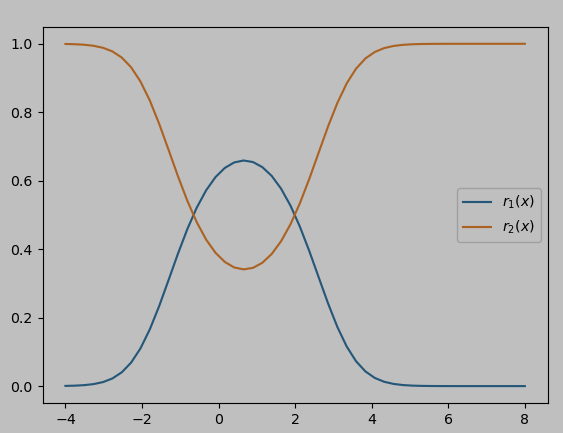
\includegraphics[width=0.8\textwidth]{Images/1b.png}
		            \end{center}

		      \item Let $B\teq \{x : r_2(x) > r_1(x)\}$. Find the set $B$.

		            \color{blue}
		            \begin{align*}
			            B & = \{x : r_2(x) > r_1(x)\}                                                                                                                      \\
			              & = \{x : 0.55 \frac{f_2(x)}{f(x)} > 0.45 \frac{f_1(x)}{f(x)}\}                                                                                  \\
			              & = \{x : 0.55 f_2(x) > 0.45 f_1(x)\}                                                                                                            \\
			              & = \{x : 0.55 \frac{1}{2\sqrt{2\pi}} \exp\left(-\frac{(x - 2)^2}{8}\right) > 0.45 \frac{1}{\sqrt{2\pi}} \exp\left(-\frac{(x - 1)^2}{2}\right)\} \\
			              & = \left\{x: \exp\left(-\frac{(x - 2)^2}{8}\right) > \frac{90}{55} \exp\left(-\frac{(x - 1)^2}{2}\right)\right\}                                \\
			              & = \left\{x: -\frac{(x - 2)^2}{8} > \log\left(\frac{18}{11}\right) - \frac{(x - 1)^2}{2}\right\}                                                \\
			              & = \left\{x: -\frac{x^2 - 4x + 4}{8} > \log\left(\frac{18}{11}\right) - \frac{x^2 - 2x + 1}{2}\right\}                                          \\
			              & = \left\{x: -x^2 + 4x - 4 > 8\log\left(\frac{18}{11}\right) - 4x^2 + 8x - 4\right\}                                                            \\
			              & = \left\{x: 3x^2 - 4x > 8\log\left(\frac{18}{11}\right)\right\}                                                                                \\
			              & \approx \boxed{\{x: x < -0.341\} \cup \{x: x > 1.674\}}
		            \end{align*}
		            \color{black}
	      \end{enumerate}


	      \pagebreak

	      %%%%%%%%%%%%%%%%%%%%%%%%%%
	      %			Problem 
	      %%%%%%%%%%%%%%%%%%%%%%%%%%
	\item {\bf Optimal and sub-optimal classifiers.} Problem 1 continued: Consider the family of classifiers
	      \[ h_t(X) = 1+\ind_{X > t} = \begin{cases} 2 &  \text{if $X > t$} \\ 1 & \text{if $X \leq t$} \end{cases}  \]
	      for $t\in\mathbb{R}$.
	      \begin{enumerate}
		      \item Calculate\footnote{This refers to the distribution over $(X,Y)$ defined in Problem 1. You will need the cumulative distribution function (cdf) of a normal random variable, which you can get in Matlab with {\tt normcdf}.} the error probabilities $\Prob(h_{1.5}(X)\neq Y|Y=1)$ and $\Prob(h_{1.5}(X)\neq Y|Y=2)$.

		            \color{blue}
		            \begin{align*}
			            \P(h_{1.5}(X) \neq Y \; | \; Y = 1) & = \P(h_{1.5}(X) = 2 \; | \; Y = 1) = \P(X > 1.5 \; | \; Y = 1) = 1 - \int_{-\infty}^{1.5} f_1(x) \; dx \approx \boxed{0.3085} \\
			            \P(h_{1.5}(X) \neq Y \; | \; Y= 2)  & = \P(h_{1.5}(X) = 1 \; | \; Y= 2) = \P(X \leq 1.5 \; | \; Y= 2) = \int_{-\infty}^{1.5} f_2(x) \; dx \approx \boxed{0.4013}
		            \end{align*}
		            \color{black}

		      \item Calculate the classification error rate $\Prob(h_{1.5}(X)\neq Y)$.

		            \color{blue}
		            \begin{align*}
			            \P(h_{1.5}(X) \neq Y) & = \P(h_{1.5}(X) \neq Y \; | \; Y = 1) \P(Y = 1) + \P(h_{1.5}(X) \neq Y \; | \; Y = 2) \P(Y = 2) \\
			                                  & = 0.45 \cdot \P(X > 1.5 \; | \; Y = 1) + 0.55 \cdot \P(X \leq 1.5 \; | \; Y = 2)                \\
			                                  & \approx 0.45 \cdot 0.3085 + 0.55 \cdot 0.4013                                                   \\
			                                  & \approx \boxed{0.3596}
		            \end{align*}
		            \color{black}

		      \item {\color{blue} (Do not submit.)} Generate $n=10^6$ iid pairs $(X_1,Y_1),(X_2,Y_2),\dotsc,(X_n,Y_n)$ from this distribution and find the fraction of times that $h_{1.5}(X_k)\neq Y_k$. Report your results. If your answer is not very close to part (b), then something is wrong.
		      \item Find another value of $t\neq 1.5$ so that the classifier $h_t$ has smaller classification error rate than $h_{1.5}$. Compute the two error probabilities from part (a) and the classification error rate from part (b) for your improved classifier.

		            \color{blue}
		            For $\boxed{t = 2}$,
		            \begin{align*}
			            \P(h_2(X) \neq Y \; | \; Y = 1) & = 1 - \int_{-\infty}^2 f_1(x) \; dx \approx \boxed{0.1587} \\
			            \P(h_2(X) \neq Y \; | \; Y = 2) & = \int_{-\infty}^2 f_2(x) \; dx \approx \boxed{0.5}        \\
			            \P(h_2(X) \neq Y)               & \approx \boxed{0.3464} < 0.3596 = \P(h_{1.5}(X) \neq Y)
		            \end{align*}
		            \color{black}

		      \item Find the classifier $h^*$ (not necessarily of the form $h_t$ above) that has the smallest possible classification error rate.

		            \color{blue}
		            Bayes' Rule tells us that
		            \[h^*(x) = \argmax_{i=1:c} \P(Y = i \; | \; X = x)\]

		            For $Y \in \{1, 2\}$,
		            \begin{align*}
			            \P(Y = 1 \; | \; X = x) & = \frac{\P(Y = 1) \P(X = x \; | \; Y= 1)}{\P(X = x)} \\
			                                    & = \frac{0.45 f_1(x)}{f(x)}                           \\
			            \P(Y = 2 \; | \; X = x) & = \frac{\P(Y = 2) \P(X = x \; | \; Y= 2)}{\P(X = x)} \\
			                                    & = \frac{0.55 f_2(x)}{f(x)}
		            \end{align*}

		            Hence,
		            \[h^*(x) = \begin{cases}
				            2 & \text{if } 0.45 f_1(x) < 0.55 f_2(x) \\
				            1 & \text{otherwise}
			            \end{cases}\]
		            \color{black}

		      \item Compute the two error probabilities from part (a) and the classification error rate from part (b) for $h^*$.

		            \color{blue}
		            \begin{align*}
			            \P(h^*(X) \neq Y \; | \; Y = 1) & = \P(h^*(X) = 2 \; | \; Y = 1)                                         \\
			                                            & = \P(0.45 f_1(X) < 0.55 f_2(X) \; | \; Y = 1)                          \\
			                                            & = \P(X \leq t \; | \; Y= 1) \qquad \text{for } 0.45f_1(t) = 0.55f_2(t) \\
			            \P(h^*(X) \neq Y \; | \; Y = 2) & = \P(h^*(X) = 1 \; | \; Y = 2)                                         \\
			                                            & = \P(X > t \; | \; Y = 2) \qquad \text{for } 0.45 f_1(t) = 0.55f_2(t)
		            \end{align*}

		            We saw in Problem 1.c that
		            \[0.45 f_1(t) = 0.55f_2(t) \iff 3t^2 - 4t - 8\log(\frac{18}{11}) = 0 \iff t = \frac{4 \pm \sqrt{16 + 96\log \frac{18}{11}}}{6}\]

		            But as we saw in Part d, we want
		            \[t = \frac{4 + \sqrt{16 + 96\log \frac{18}{11}}}{6} \approx 1.992\]
		            so
		            \begin{align*}
			            \P(h^*(X) \neq Y \; | \; Y = 1) & =  \int_{-\infty}^t f_1(x)\; dx \approx \boxed{0.1605}                                               \\
			            \P(h^*(X) \neq Y \; | \; Y = 2) & =  1 - \int_{-\infty}^{t} f_2(x)\; dx \approx \boxed{0.4985}                                         \\
			            \P(h^*(X) \neq Y)               & = 0.45 \P(h^*(X) \neq Y \; | \; Y = 1) + 0.55 \P(h^*(X) \neq Y \; | \; Y = 2) \approx \boxed{0.3464}
		            \end{align*}
		            \color{black}
	      \end{enumerate}


	      \pagebreak

	      %%%%%%%%%%%%%%%%%%%%%%%%%%
	      %			Problem 
	      %%%%%%%%%%%%%%%%%%%%%%%%%%
	\item {\bf Preprocessing cannot improve optimal classification performance.} Consider a pair of random variables $(X,Y)$ where $Y\in\{1,\dotsc,s\}$. Let $L$ be the optimal classification error rate for predicting $Y$ from $X$. Suppose we transform $X$ into $\tilde X=g(X)$ for some function $g$, and predict $Y$ using $\tilde X$ instead of $X$. In other words, we preprocess the data prior to classification. Let $\tilde L$ be the optimal classification error rate for predicting $Y$ from $\tilde X$.
	      \begin{enumerate}
		      \item Prove that $\tilde L \geq L$, i.e., preprocessing can only create more error if we are using the optimal
		            classifier.\footnote{This result is analogous to the data processing inequality in information theory (if you've seen that before), which says that the mutual information between $Y$ and $\tilde X$ is less than or equal to the mutual information between $Y$ and $X$. At \underline{best}, preprocessing loses no information.}

		            \color{blue}
		            Let $\tilde h$ be the optimal classifier for predicting $Y$ from $\tilde X$ and $h$ be the optimal classifier for predicting $Y$ from $X$. By Bayes' Rule, we can write
		            \begin{align*}
			            L        & = \P(h(X) \neq Y) = 1 - \P(h(X) = Y)                   \\
			                     & = 1 - \int_x \P(Y = h(x) \; | \; X = x) f(x)\; dx      \\
			                     & = 1 - \int_x \max_c \P(Y = c \; | \; X = x) f(x)\; dx  \\
			                     & = 1 - \E_X[\max_c \P(Y = c \; | \; X)]                 \\
			            \tilde L & = 1 - \E_{\tilde X}[\max_c \P(Y = c \; | \; \tilde X)]
		            \end{align*}

		            Hence, it suffices to show
		            \begin{align*}
			            \E_{\tilde X} [\max_c \P(Y = c \; | \; \tilde X)] & \leq \E_{X} [\max_c \P(Y = c \; | \; X)] \\
			            \E_{g(X)} [\max_c \P(Y = c \; | \; g(X))]         & \leq \E_{X} [\max_c \P(Y = c \; | \; X)]
		            \end{align*}

		            Notice,
		            \begin{align*}
			            \P(Y = c \; | \; g(X)) & = \E[\ind_{Y = c} \; | \; g(X)] \\
			            \P(Y = c \; | \; X)    & = \E[\ind_{Y = c} \; | \; X]
		            \end{align*}
		            so
		            \begin{align*}
			            \E [\P(Y = c \; | \; X) \; | \; g(X)] & = \E[\E[\ind_{Y = c} \; | \; X] \; | \; g(X)] \\
			                                                  & = \P(Y = c \; | \; g(X))
		            \end{align*}

		            But since $\max$ is a convex function, we can apply Jensen's inequality to get
		            \begin{align*}
			            \max_c \P(Y = c \; | \; g(X)) & = \max_c \E[\P(Y = c \; | \; X) \; | \; g(X)]    \\
			                                          & \leq \E[\max_c \P(Y = c \; | \; X) \; | \; g(X)] \\
		            \end{align*}

		            Taking expected values,
		            \begin{align*}
			            \E[\max_c \P(Y = c \; | \; g(X)) ] & \leq \E[\E[\max_c \P(Y = c \; | \; X) \; | \; g(X)]] \\
			                                               & = \E[\max_c \P(Y = c \; | \; X]]                     \\
			            1 - \tilde L                       & \leq 1 - L
		            \end{align*}
		            hence, $\tilde L \geq L$.

		            \color{black}
		      \item Prove that $\tilde L = L$ if the function $g$ is invertible.

		            \color{blue}
		            Suppose $g$ is invertible.

		            In part (a), we showed that for any $g: x \mapsto g(X)$,
		            \[1 - \tilde L = \E[\max_c \P(Y = c \; | \; g(X))] \leq \E[\max_c \P(Y = c \; | \; X)] = 1 - L \]

		            However, by assumption, $\exists g^{-1}$ such that $g^{-1}(g(X)) = X$ so we can apply the same argument to $g^{-1}$ to get
		            \[\E[\max_c \P(Y = c) \; | \; g^{-1}(g(X))] \leq \E[\max_c \P(Y = c \; | \; g(X))]\]
		            but since $g^{-1}(g(X)) = X$, we have
		            \begin{align*}
			            \begin{cases}
				            \E[\max_c \P(Y = c) \; | \; X] \leq \E[\max_c \P(Y = c \; | \; g(X))] \\
				            \E[\max_c \P(Y = c \; | \; g(X))] \leq \E[\max_c \P(Y = c \; | \; X)]
			            \end{cases} & \implies \E[\max_c \P(Y = c) \; | \; X] = \E[\max_c \P(Y = c \; | \; X)]                              \\
			                                                                                     & \implies 1 - \tilde L = 1 - L            \\
			                                                                                     & \implies \tilde L = L \quad \blacksquare
		            \end{align*}



		            \color{black}

		      \item Suppose that $s=2$ and that the class conditional distributions for $X$ given $Y$ have pdfs $f_1(x)$ and $f_2(x)$ over $\mathbb{R}^d$. Suppose that $g$ is invertible and that both $g$ and $g^{-1}$ are continuously differentiable. Let $\tilde f_1(\tilde x)$ and $\tilde f_2(\tilde x)$ be the class conditional pdfs of $\tilde X$ given $Y$.\footnote
		            {
		            {\bf Change of variables/change of densities.} Let
		            $g:A\subseteq \mathds{R}^d \to B \subseteq\mathds{R}^d$ be invertible and onto (i.e. $\forall \tilde{x}\in B$, $\exists x\in A$ such that $g(x) = \tilde{x}$) and let $g^{-1}$ be the inverse of $g$. Suppose that both $g$ and $g^{-1}$ are continuously differentiable. If $X$ is a random vector taking values in $\mathds{R}^d$ and having density $f_X$, then what is the density of $\tilde{X}\doteq
			            g(X)$? This is just a change of variables problem, as follows:
		            \[
			            f_X(x)dx =\ \ \text{(c.o.v. $x=g^{-1}(\tilde{x})$)}\ \
			            f_X\left(g^{-1}(\tilde{x})\right)
			            \left|\frac{dx}{d\tilde{x}}\right|d\tilde{x}
			            = f_X\left(g^{-1}(\tilde{x})\right)
			            \left|\det J^{g^{-1}}(\tilde{x})\right|d\tilde{x}
		            \]
		            where $J^{g^{-1}}$ is the $d\times d$ Jacobian matrix, with $i,j$ entry
		            $\frac{\partial g_i^{-1}(\tilde{x})}{\partial \tilde{x}_j}$, and $g_i^{-1}$ is the $i$ component of $g^{-1}(\tilde{x})\in\mathds{R}^d$.
		            Therefore, for any $S\subseteq A$
		            \[
			            \int_{x\in S} f_X(x)dx
			            = \int_{\tilde{x}\in g(S)} f_X\left(g^{-1}(\tilde{x})\right)
			            \left|\det J^{g^{-1}}(\tilde{x})\right|d\tilde{x}
			            \Longrightarrow f_{\tilde{X}}(\tilde{x}) =
			            f_X\left(g^{-1}(\tilde{x})\right)
			            \left|\det J^{g^{-1}}(\tilde{x})\right|
		            \]
		            Or in the other direction,
		            $\displaystyle
			            f_X(x) =
			            f_{\tilde{X}}\left(g({x})\right)
			            \left|\det J^{g}(x)\right|
		            $. Notice then that $\displaystyle \left|\det J^{g}(x)\right|
			            =\frac{1}{\left|\det J^{g^{-1}}\left(g(x)\right)\right|}$, which makes sense for an area element.
		            Notice also that therefore the smoothness conditions on $g$ and its inverse imply, among other things, that the Jacobian determinant is everywhere non-zero.
		            }
		            Show that the Neyman-Pearson classifiers for $Y$ given $X$ and for $Y$ given $\tilde{X}$ produce the same ROC curves.

		            \color{blue}
		            Let
		            \begin{align*}
			            h_t(X)               & = \begin{cases}
				                                     1 & \text{if } \frac{f_2(X)}{f_1(X)} < t \\
				                                     2 & \text{otherwise}
			                                     \end{cases}                             \\
			            \tilde h_t(\tilde X) & = \begin{cases}
				                                     1 & \text{if } \frac{\tilde f_2(\tilde X)}{\tilde f_1(\tilde X)} < t \\
				                                     2 & \text{otherwise}
			                                     \end{cases}
		            \end{align*}

		            Then for all $t$, we want
		            \[\frac{\P(\tilde h_t(\tilde X) = 2 \; | \; Y = 2)}{\P(\tilde h_t(\tilde X) = 2 \; | \; Y = 1)} = \frac{\P( h_t( X) = 2 \; | \; Y = 2)}{\P( h_t(X) = 2 \; | \; Y = 1)}\]

		            It suffices to show that, for all $t$, $h_t(X) = \tilde h_t(\tilde X)$ or equivalently
		            \[\frac{f_2(X)}{f_1(X)} < t \iff \frac{\tilde f_2(\tilde X)}{\tilde f_1(\tilde X)} < t \]

		            However, by the change of variables formula, we know that
		            \[\frac{\tilde f_2(\tilde X)}{\tilde f_1(\tilde X)} = \frac{f_2(g^{-1}(\tilde X)) \abs{\det J^{g^{-1}}(\tilde X)}}{f_1(g^{-1}(\tilde X)) \abs{\det J^{g^{-1}}(\tilde X)}} = \frac{f_2(g^{-1}(\tilde X))}{f_1(g^{-1}(\tilde X))} = \frac{f_2(g^{-1}(g(X)))}{f_1(g^{-1}(g(X)))} = \frac{f_2(X)}{f_1(X)}\]
		            which gives us the strictly stronger result that for $g$ invertible and $g, g^{-1} \in C^1$,
		            \[\frac{\tilde f_2(\tilde X)}{\tilde f_1(\tilde X)} = \frac{f_2(X)}{f_1(X)} \implies \tilde h_t(\tilde X) = h_t(X) \implies \frac{\P(\tilde h_t(\tilde X) = 2 \; | \; Y = 2)}{\P(\tilde h_t(\tilde X) = 2 \; | \; Y = 1)} = \frac{\P( h_t( X) = 2 \; | \; Y = 2)}{\P( h_t(X) = 2 \; | \; Y = 1)} \]
		            for all values of $t$. Hence, the Neyman-Pearson classifiers for $Y$ given $X$ and for $Y$ given $\tilde{X}$ produce the same ROC curves.

		            \color{black}
	      \end{enumerate}

	      {\em Remark}: Preprocessing, i.e., finding good features, is often crucial for real-world classification, even though you just showed that it can only hurt optimal performance. The reason is that in most practical situations we do not know the underlying distributions and, consequently, we cannot do optimal classification. Preprocessing can make it easier for a statistical procedure to learn a good classifier, even though the classifier may not be optimal.


	      \pagebreak


	      %%%%%%%%%%%%%%%%%%%%%%%%%%
	      %			Problem 
	      %%%%%%%%%%%%%%%%%%%%%%%%%%
	\item {\color{blue} (Do not submit.)} {\bf Constructing the ROC curve.} Consider a two-category classification problem for $(X,Y)$ where $X\in\mathbb{R}^2$ and $Y\in\{1,2\}$ with $\pi_1\teq\Prob(Y=1)=0.4$ and $\pi_2\teq\Prob(Y=2)=0.6$.  We will describe the distribution of $X=(X_1,X_2)$ in terms of polar coordinates $(R,U)$ that satisfy
	      \[ (X_1,X_2) = (R\cos U,R\sin U) \]
	      or, equivalently,  \[ (R,U) = (\sqrt{X_1^2+X_2^2}, \text{atan2}(X_2,X_1)) . \]
	      Conditional on $Y=1$, $R$ and $U$ are independent with $R\sim $ Gamma$(20,0.1)$ and $U\sim $ Uniform$(0,2\pi)$.  Conditional on $Y=2$, $R$ and $U$ are independent with $R=\sqrt{2E}$ for $E\sim $ Exponential$(1)$ and \newline
	      $U\sim $ Uniform$(0,2\pi)$.\footnote{Gamma$(a,b)$ has pdf
	      \[ f(x;a,b) \teq \frac{1}{b^a\Gamma(a)}x^{a-1}\exp(-x/b)\ind\{x\geq 0\}
	      \]
	      and you can use the Matlab function {\tt gamrnd(a,b,m,n)} to generate an $m\times n$ array of iid gamma$(a,b)$ random variables.
	      (This is just one of several parameterizations that are commonly used for the Gamma distribution.)
	      Exponential$(c)$ has pdf
	      \[ f(x;c) \teq \frac{1}{c}\exp(-x/c)\ind\{x\geq 0\}
	      \]
	      and you can use the Matlab function {\tt exprnd(c,m,n)} to generate an $m\times n$ array of iid exponential$(c)$ random variables.}
	      \begin{enumerate}
		      \item Sample $1000$ iid pairs from this distribution and make three scatter plots: (i) $X|Y=1$, (ii) $X|Y=2$, and (iii) $X$ for any $Y$, but with different symbols for the two different classes.  $X|Y=1$ should be a noisy ring and $X|Y=2$ should be a noisy disk and they should overlap significantly.
		      \item Let $f_1(r,u)$ and $f_2(r,u)$ denote the conditional pdfs of $(R,U)$ given $Y=1$ and given $Y=2$, respectively.  Derive expressions for $f_1$ and $f_2$.  Find an expression for the family of Neyman-Pearson classifiers, say $(h_t : 0 < t < \infty)$ using $f_1$ and $f_2$.  Is this the same family of classifiers that you would have derived if you had used rectangular coordinates instead of polar coordinates?  Why or why not?
		      \item (Approximately) compute and plot the optimal ROC curve traced out by the family of Neyman-Pearson classifiers.  Do this by generating $n=10^5$ iid samples from $(X,Y)$, called the {\em test data set}, and estimating the DR (detection rate) and FAR (false alarm rate) for each $h_t$ as you vary $t$ to trace out the ROC curve.\footnote{You should only create a single test data set, i.e., you should use the same test data set for each $h_t$: For each $t$, you compute $h_t$ on all $10^5$ feature vectors ($X$) and compare $h_t$ to the true class labels ($Y$) to approximate DR and FAR. One issue is how to choose an appropriate grid of $t$ values. A good strategy is to first compute $f_2/f_1$ on all $10^5$ test data points, sort the ratios, and choose every 100th value, to get a list of $1000$ candidate values of $t$. Include the values $-\infty$ and $\infty$ in your list of $t$ to get the points $(1,1)$ and $(0,0)$ on your ROC curve. Linearly interpolate points on the ROC curve so that you draw a smooth curve.}
		      \item Approximately, what is the optimal classification error rate, i.e, $\inf_h \Prob(h(X)\neq Y)$, where the infimum is taken over all possible classifiers?  What classifier achieves this optimal error rate?
	      \end{enumerate}


	      \pagebreak

	      %%%%%%%%%%%%%%%%%%%%%%%%%%
	      %			Problem 
	      %%%%%%%%%%%%%%%%%%%%%%%%%%

	\item {\color{blue} (Do not submit.)} {\bf Information versus the curse of dimensionality.} Now we will modify the distribution in problem 4 by increasing the dimensionality of the feature space from 2 to $d$.  The distribution of $(X_1,X_2)$ remains the same.  Conditional on $Y=c$, $(X_3,\dotsc,X_d)$ are (conditionally) independent with $X_i\sim $ Normal$(c/i,1)$.  (Note that each new feature adds discriminatory power, because its distribution is different for each class, but that the amount of discriminatory power is decreasing.  This is a fairly common situation for high-dimensional data.)
	      \begin{enumerate}
		      \item Let $f_1(r,u,x_3,\dotsc,x_d)$ and $f_2(r,u,x_3,\dotsc,x_d)$ denote the conditional pdfs of $(R,U,X_3,\dotsc,X_d)$ given $Y=1$ and given $Y=2$, respectively.  Derive expressions for $f_1$ and $f_2$.  Find an expression for the family of Neyman-Pearson classifiers, $\{(h_t : 0 < t < \infty\}$, using $f_1$ and $f_2$.  Is this the same family of classifiers that you would have derived if you had used $X_{1:d}$ instead of $R,U,X_{3:d}$?  Why or why not?
		      \item Repeat Problem 4c,d for the cases $d=5$, $d=50$, $d=200$.
	      \end{enumerate}


	      \pagebreak

	      %%%%%%%%%%%%%%%%%%%%%%%%%%
	      %			Problem 
	      %%%%%%%%%%%%%%%%%%%%%%%%%%

	\item {\color{blue} (Do not submit.)} {\bf Bias and variance in the $\mathbf{k}$-nearest neighbor classifier.}
	      On this problem you will compute the ROC curve for a $k$-nearest neighbor classifier on the same data distribution, but pretending that this  distribution is {\em unknown}.
	      Except for reproducing the optimal ROC curve from Problems 4 and 5, you should not use the true data distribution in this problem. In practice, for statistical classification, the true data distribution is unknown.

	      Download the text files {\tt X.dat} and {\tt Y.dat} that are posted with this HW.\footnote{You can load these files into Matlab with the commands {\tt load X.dat} and {\tt load Y.dat}. The $2000{\times}200$ matrix {\tt X} and the $2000{\times}1$ vector {\tt Y} will be in your workspace.} The file {\tt X.dat} contains an $m\times d$ matrix of $m=2000$ iid samples of $X$ using $d=200$. The file {\tt Y.dat} contains an $m\times 1$ vector of $m=2000$ iid samples of $Y$. The $i$th rows of {\tt X.dat} and {\tt Y.dat} are paired, giving a joint sample of $(X,Y)$, for $i=1,\dotsc,m$.

	      When testing the performance of a statistical classifier, it is of the utmost importance to \underline{use separate datasets} \underline{for training and testing}. So the first thing you should do is partition the downloaded data {\tt X} and {\tt Y} into a {\em training} dataset and a {\em testing} dataset. Use rows $1,\dotsc,1000$ for the training dataset and rows $1001,\dotsc,2000$ for the testing dataset. In parts of this problem you will investigate how performance varies with the amount of training data $n$, in which case you will use subsets of size $n$ from the training dataset for training ($n$ will never be more than $1000$). Regardless of the amount of training data, use all $1000$ rows of the testing data for testing (i.e., rows $1001,\dotsc,2000$ of the downloaded data).

	      Building a $k$-nearest neighbor classifier in Matlab is easy. First you train the model using only the training data:
	      \begin{verbatim}
 Xtrain = X(1:n,1:d); 
 Ytrain = Y(1:n);
 mdl = fitcknn(Xtrain,Ytrain,'NumNeighbors',k);
 \end{verbatim}
	      The function {\tt fitcknn} trains the model (which for a $k$-NN classifier involves, at most, computing a data structure to facilitate searching later for neighbors). The first argument is the feature vector data arranged as an $n\times d$ matrix, where $n$ is the number of training points and $d$ is the number of feature dimensions. Since you are varying both $n$ and $d$ in this problem, you will need to specify them ahead of time. The second argument is the class label data arranged as an $n\times 1$ vector, where the $i$th label corresponds to the $i$th row of the training data. There are many optional arguments, but the only one that you will vary is the number of neighbors $k$.

	      Once you have trained the model and stored it in a variable (called {\tt mdl} above), then you can use it to predict the label of new data like this: {\tt yhat = predict(mdl,x)}, where {\tt x} is a new feature vector and {\tt yhat} is the predicted label. The default prediction uses majority voting (to approximate the Bayes classifier), but this only corresponds to a single point on the ROC curve. In this problem you want to approximate the entire curve. A $k$-NN classifier traces out an ROC curve by varying the fraction $t$ of the $k$ neighbors that need to be class $2$ in order for the classifier to guess $Y=2$. So, instead of using the {\tt predict} function to actually predict, we will use it to get the $k$-NN approximation $\hat r_{c,k}(x)$, which is exactly the fraction of neighbors in each class. This is given by the second output argument of {\tt predict}:
	      \begin{verbatim}
 Xtest = X(1001:2000,1:d);
 Ytest = Y(1001:2000);
 [~,rhat] = predict(mdl,Xtest); 
 \end{verbatim}
	      (This symbol \verb|~| is tilde.) Note that we are predicting for the observations in the {\em testing} data, not the training data that we used for {\tt mdl} (as long as $n\leq 1000$). We are also simultaneously predicting on all $1000$ testing points; there is no need to loop over the testing points and separately predict on each one. The output {\tt rhat} will be a $1000\times 2$ matrix, where {\tt rhat(i,c)} gives $\hat r_{c,k}(x)$ ($x$ being the $i$th testing data point). Once you know $\hat r_{c,k}$, you can build a family of classifiers by varying the threshold for when to guess class $2$ versus class $1$ as you compare $\hat r_{2,k}$ to $\hat r_{1,k}$.

	      \begin{enumerate}
		      \item (Approximately) compute the ROC curve for the $k$-nearest neighbor classifier using this training data for the first $d=2$ features.\footnote{You proceed the same way as Problems 4c and 5b, especially footnote 5, except that instead of a classifier based on comparing $f_2/f_1$ to a threshold, you compare the fraction of $k$-nearest neighbors that are class 2 to a threshold.  This fraction is given in the second column of {\tt rhat}. (Also, you do not need to generate your own training or testing data --- use the appropriate part of the downloaded data as indicated above.)  Linearly interpolate points on the ROC curve so that you draw a continuous curve. This is especially important for small $k$, since there are only $k+2$ meaningful thresholds.} Do this for each of $k=1,5,21,101,501$. Draw the five curves all on the same plot together and with the optimal ROC curve that you computed in Problems 4 and 5.  Now repeat for the cases $d=5$, $d=50$, and $d=200$. (When you are done, you should have 4 plots, each with 6 ROC curves on it. Make sure that all of the plots and curves are clearly labeled.)
		      \item Repeat part (a) using $n=200$ training points. (Using $k > n$ is equivalent to using $k=n$.)

		      \item Concerning the results from (a) and (b), what (if any) trends do you find when: (i) fixing $d$ and $k$ and varying $n$; (ii) fixing $k$ and $n$ and varying $d$; and (iii) fixing $n$ and $d$ and varying $k$? Use the analyses developed in the lecture on $k$-nearest neighbor classifiers (especially vis-a-vis bias and variance and the effects of $n$ and $k$ on the radius $R_k(x)$) to interpret the three trends. (Concerning (ii), it might help to think about the effect of added dimensions on the distances between training points.)

	      \end{enumerate}

	      \pagebreak


	      %%%%%%%%%%%%%%%%%%%%%%%%%%
	      %			Problem 
	      %%%%%%%%%%%%%%%%%%%%%%%%%%

	\item {\bf Parametrization, over parametrization, and decision surfaces.}
	      Consider a classification problem for feature vectors $x\in\mathds{R}^d$ with $s$ categories, $Y\in\{1,2,\ldots,s\}$.
	      \begin{enumerate}[(a)]

		      \item Here is a common way to write the softmax model for $r_c(x) \triangleq \Prob(Y=c | x) = \Exp[\ind_{Y=c} | x]$:
		            \begin{equation}
			            \label{eqn:over_parametrized}
			            r_c(x) = \frac{e^{\beta_c\cdot x}}{\sum_{\tilde{c}=1}^s e^{\beta_{\tilde{c}}\cdot x}} \quad \forall\ c=1:s
		            \end{equation}
		            where $\beta_c\in\mathds{R}^d$ for each $c=1:s$.
		            Define $\tilde{\beta}_c = \beta_c-\beta_1$ for each $c=2:s$, and show that: %, let $\tilde{\beta}_1 = (0,0,\ldots,0)$ be the zero vector in $R^d$. 
		            \[
			            \tilde{r}_c(x) \triangleq \begin{cases}  \frac{e^{\tilde{\beta}_c \cdot x}}{1+\sum_{\tilde{c}=2}^s e^{\tilde{\beta}_{\tilde{c}}\cdot x}} &
               c=2:s                                                                                             \\  \\
               \frac{1}{1+\sum_{\tilde{c}=2}^s e^{\tilde{\beta}_{\tilde{c}}\cdot x}}                           &
               c=1
			            \end{cases}
		            \]
		            gives the exact same classifier as in (\ref{eqn:over_parametrized}), but with $d$ fewer parameters. (In other words, (\ref{eqn:over_parametrized}) is ``over parametrized," albeit less burdened by notation.)


		            \color{blue}
		            First consider the case $c \neq 1$. We have
		            \begin{align*}
			            \tilde r_c(x) & = \frac{e^{\tilde \beta_c \cdot x}}{1 + \sum_{\tilde c = 2}^s e^{\tilde \beta_{\tilde c} \cdot x}}                       \\
			                          & = \frac{e^{\beta_c \cdot x - \beta_1 \cdot x}}{1 + \sum_{\tilde c = 2}^s e^{\beta_{\tilde c} \cdot x - \beta_1 \cdot x}} \\
			                          & = \frac{e^{\beta_c \cdot x}}{e^{\beta_1 \cdot x} + \sum_{\tilde c = 2}^s e^{\beta_{\tilde c} \cdot x}}                   \\
			                          & = \frac{e^{\beta_c \cdot x}}{\sum_{\tilde c = 1}^s e^{\beta_{\tilde c} \cdot x}} = r_c(x)
		            \end{align*}
		            so indeed $\tilde r_c(x) = r_c(x)$ for all $c=2:s$.

		            Now we take the case $c = 1$. Notice
		            \[\sum_{c=1}^s \tilde r_c(x) = \sum_{c=1}^s r_c(x) = \sum_{c=1}^{s} \P(Y = c \; | \; x) = 1\]
		            so we must also have
		            \begin{align*}
			            \tilde r_1(x) & = 1 - \sum_{c=2}^s \tilde r_c(x)                        \\
			                          & = 1 - \sum_{c=2}^s r_c(x) \qquad (\text{by first case}) \\
			                          & = r_1(x)
		            \end{align*}

		            Finally, $r_c(x)$ has $sd$ parameters ($\{\beta_c\}_{c = 1:s}, \beta_i \in \R^d$) while $\tilde r_c(x)$ has only $(s-1)d$ parameters ($\{\tilde \beta_c\}_{c = 2:s}, \tilde \beta_i \in \R^d$) so we conclude that $\tilde r_c(x)$ is a reparametrization of $r_c(x)$ with $d$ fewer parameters.

		            \color{black}


		      \item There is yet another common representation of softmax in which a constant offset, or ``bias", is added to each
		            exponent, e.g.
		            \[
			            {r}_c(x) \triangleq \begin{cases}  \frac{e^{\alpha_c+\beta_{c}\cdot x}}{1+\sum_{\tilde{c}=2}^s e^{\alpha_c+\beta_{\tilde{c}}\cdot x}} &
               c=2:s                                                                                                \\ \\
               \frac{1}{1+\sum_{\tilde{c}=2}^s e^{\alpha_{\tilde{c}} + \beta_{\tilde{c}}\cdot x} }                &
               c=1
			            \end{cases}
		            \]

		            Consider the minimum-error (``Bayesian") classifier
		            \begin{equation}
			            \label{eqn:Bayes}
			            h^*(x) \triangleq \text{argmax}_{c=1:s} r_c(x)
		            \end{equation}
		            Assume that $d\geq s-1$ and that each of $\beta_2,\beta_3,\ldots\beta_s$ are distinct. Show that all of the $ {s}\choose{2}$ decision surfaces share an affine subspace of dimension at least
		            $d-s + 1$ or their intersection is empty.

		            Point: Despite what I drew in class, the categories defined by $h^*$ form conical-like regions emanating from a common affine hyperplane. By ``conical-like," I mean cones with boundaries replaced by a collection of flat surfaces.  So, for example, if $d=2$ and $s=3$, then the decision boundaries are three lines passing through a common point.


		            \color{blue}
		            For the optimal classifier $h^*$, we have $s$ surfaces given by
		            \[\left\{\frac{1}{1 + \sum_{\bar c =2}^{s} \exp(\alpha_{\bar c} + \beta_{\bar c} \cdot x)}, \frac{\exp(\alpha_2 + \beta_2 \cdot x)}{1 + \sum_{\bar c}^{s} \exp(\alpha_{\bar c} + \beta_{\bar c} \cdot x)}, \dots,\frac{\exp(\alpha_s + \beta_s \cdot x)}{1 + \sum_{\bar c}^{s} \exp(\alpha_{\bar c} + \beta_{\bar c} \cdot x)} \right\}\]

		            Then the decision boundaries are given by the intersection $B_{ij}$ of any two of the $s$ surfaces $i, j$ -- clearly there are $\binom{s}{2}$ such intersections.

		            We are interested in the intersection of all such precision boundaries, $\bigcap_{i, j=1:s} B_{ij}$.

		            For any two surfaces $i,j$, we have
		            \begin{align*}
			            B_{ij} & = \{x \in \R^d \; | \; r_i(x) = r_j(x)\}                                                                                                                                                                                                                                \\
			                   & =\left\{x \in \R^d \big\vert \; \frac{\exp(\alpha_i + \beta_i \cdot x)}{1 + \sum_{\bar c =2}^{s} \exp(\alpha_{\bar c} + \beta_{\bar c} \cdot x)}, \frac{\exp(\alpha_j + \beta_j \cdot x)}{1 + \sum_{\bar c}^{s} \exp(\alpha_{\bar c} + \beta_{\bar c} \cdot x)}\right\} \\
			                   & = \{x \in \R^d \; | \; \alpha_i + \beta_i \cdot x = \alpha_j + \beta_j \cdot x\}                                                                                                                                                                                        \\
			                   & = \{x \in \R^d \; | \; (\beta_i - \beta_j) \cdot x = \alpha_j - \alpha_i\}
		            \end{align*}

		            Hence,
		            \[\bigcap_{i, j} B_{ij} = \left\{x: x \cdot \left(\beta_1 - \sum_{c = 2}^s \beta_c\right)  = 1 - \sum_{c=2}^{s} \alpha_c \right\}\]
		            which corresponds precisely to the solution of the linear system of equations with $(s - 1)$ equations and $d$ variables. By assumption, $d \geq s - 1$, so the solution space is at least $d - (s - 1) = d - s + 1$ dimensional.


		            \color{black}


	      \end{enumerate}


	      \pagebreak

	      %%%%%%%%%%%%%%%%%%%%%%%%%%%%%%% 2610

	\item[] \hspace{-3ex} {\bf For 2610 or for extra credit:}





	      %%%%%%%%%%%%%%%%%%%%%%%%%%
	      %			Problem 
	      %%%%%%%%%%%%%%%%%%%%%%%%%%

	\item {\bf Non-deterministic classifiers.} A non-deterministic classifier is allowed to make a stochastic prediction using an independent source of randomness. For example, we might have a Neyman-Pearson classifier that predicts $Y=2$ if $f_2(x)>f_1(x)$ and predicts $Y=1$ if $f_1(x)>f_2(x)$, but randomly chooses between $Y=1,2$ when $f_1(x)=f_2(x)$. The performance of a non-deterministic classifier is computed by averaging over its internal source of randomness. Consider two classifiers $h_0$ and $h_1$ with false alarm rates and detection rates given by $(\text{FAR}_0,\text{DR}_0)$ and $(\text{FAR}_1,\text{DR}_1)$, respectively. Consider a non-deterministic classifier $h_\alpha$ created by choosing $Z\sim $ Bernoulli($\alpha$) and classifying with $h_Z$, where $Z$ is chosen independently every time the classifier is used. Compute the FAR and DR for $h_\alpha$.

	      \color{blue}
	      \begin{align*}
		      h_{\alpha}(x) & = \begin{cases}
			                        h_0(x) & \text{if } Z = 0 \\
			                        h_1(x) & \text{if } Z = 1
		                        \end{cases}                                                                                   \\
		      \text{FAR}    & = \P(h_{Z}(X) = 2 \; | \; Y = 1)                                                                              \\
		                    & = \P(h_1(X) = 2, Z = 1 \; | \; Y = 1) + \P(h_0(X) = 2, Z = 0 \; | \; Y = 1)                                   \\
		                    & = \P(h_1(X) = 2 \; | \; Y = 1) \P(Z = 1 \; | \; Y = 1) + \P(h_0(X) = 2 \; | \; Y = 1) \P(Z = 0 \; | \; Y = 1) \\
		                    & = \P(h_1(X) = 2 \; | \; Y = 1) \alpha + \P(h_0(X) = 2 \; | \; Y = 1) (1 - \alpha)                             \\
		                    & = \boxed{\alpha \text{FAR}_1 + (1 - \alpha) \text{FAR}_0}                                                     \\
		      \text{DR}     & = \P(h_{Z}(X) = 2 \; | \; Y = 2)                                                                              \\
		                    & = \P(h_1(X) = 2, Z = 1 \; | \; Y = 2) + \P(h_0(X) = 2, Z = 0 \; | \; Y = 2)                                   \\
		                    & = \P(h_1(X) = 2 \; | \; Y = 2) \P(Z = 1 \; | \; Y = 2) + \P(h_0(X) = 2 \; | \; Y = 2) \P(Z = 0 \; | \; Y = 2) \\
		                    & = \P(h_1(X) = 2 \; | \; Y = 2) \alpha + \P(h_0(X) = 2 \; | \; Y = 2) (1 - \alpha)                             \\
		                    & = \boxed{\alpha \text{DR}_1 + (1 - \alpha) \text{DR}_0}
	      \end{align*}
	      \color{black}



	      \pagebreak

	      %%%%%%%%%%%%%%%%%%%%%%%%%%
	      %			Problem  
	      %%%%%%%%%%%%%%%%%%%%%%%%%%


	\item {\bf Shape of the optimal ROC curve.} Consider a two-class classification problem. Let $M\subseteq[0,1]^2$ denote the set of all possible $(FAR,DR)$ pairs for this classification problem, including non-deterministic classifiers. That is,
	      \[ M = \{(f,d) : \exists \text{ a possibly non-deterministic classifier $h$ with $(\text{FAR}_h,\text{DR}_h)=(f,d)$} \}  . \]
	      \begin{enumerate}
		      \item Prove that $M$ is a convex set\footnote{A set $M$ (in a vector space) is convex if $x,y\in M$ and $\lambda\in[0,1]$ implies $\lambda x + (1-\lambda) y\in M$.} containing the points $(0,0)$ and $(1,1)$.

		      \item The optimal ROC curve is the function
		            \[ D(f) = \sup \{d : (f,d)\in M\}  , \]
		            which gives the largest possible DR over all classifiers with FAR $=f$.
		            (Recall that the $\sup$---which is short for ``supremum"---of a set is its least upper bound.)
		            Prove that $D$ is concave and non-decreasing with $D(0)\geq 0$ and $D(1)=1$. (Note: Neyman-Pearson theory tells us how to find a classifier that actually achieves $D(f)$ for each $f$, but you should not use the Neyman-Pearson Lemma in this problem, because we did not discuss the fully general case with non-deterministic classifiers and with abstract random variables that might not have pmfs or pdfs.)
	      \end{enumerate}



	      \pagebreak

	      %%%%%%%%%%%%%%%%%%%%%%%%%%
	      %			Problem 
	      %%%%%%%%%%%%%%%%%%%%%%%%%%

	\item {\bf Area under the ROC curve.} The area under the ROC curve (in the unit box $[0,1]\times[0,1]$) is a commonly used measure of performance for a family of classifiers. This problem develops a way to think about what that area means quantitatively. The cumulative distribution function (cdf) of a random variable $Z$ is $F(z)=\Prob(Z\leq z)$ and the complementary cdf (ccdf) is $G(z)=\Prob(Z > z)=1-F(z)$.
	      \begin{enumerate}
		      \item Let $Z$ be a real-valued random variable with a continuous cdf $F$ and ccdf $G$.  Define $U=F(Z)$ and $V=G(Z)$. Show that $U$ and $V$ are uniform$(0,1)$ random variables.
		      \item Let $Z_1$ and $Z_2$ be independent real-valued random variables with continuous and strictly monotonic cdf's $F_1$ and $F_2$, respectively, and ccdfs $G_1$ and $G_2$. Define the functions $\alpha(s)=F_1(F_2^{-1}(s))$ and $\beta(s)=G_2(G_1^{-1}(s))$ for $s\in(0,1)$, where, e.g., $F_2^{-1}$ is the inverse function of $F_2$. Show that
		            \[ \textstyle \Prob(Z_1\leq Z_2) = \int_0^1 \alpha(s)\; ds = \int_0^1 \beta(s) \; ds . \]
		      \item  Consider a pair of random variables $(X,Y)$ where $Y\in\{1,2\}$ and $X\in\mathcal{S}$ for some arbitrary space $\mathcal{S}$. Consider a family of classifiers $(h_t: t\in\mathbb{R})$ of the form
		            \[ h_t(x) = 1 + \ind\{g(x)\geq t\} , \]
		            where $g:\mathcal{S}\mapsto\mathbb{R}$. Define the random variable $Z=g(X)$ and the conditional cdfs $F_c(z)=\Prob(Z\leq z|Y=c)$.  Suppose that $F_1$ and $F_2$ are each continuous and strictly increasing. Let $A$ be the area under the ROC curve traced out by $h_t$ as $t$ varies over $\mathbb{R}$. Let $(X_1,Y_1)$ and $(X_2,Y_2)$ be independent copies of $(X,Y)$. Show that
		            \[ A = \Prob(g(X_1)\leq g(X_2)\mid Y_1=1,Y_2=2) . \]
	      \end{enumerate}
	      In other words, the area under the ROC curve is the probability that $g$ puts independent samples $X_1\sim \Prob(X=x|Y=1)$ and $X_2 \sim \Prob(X=x|Y=1)$ ``in the right order.''

	      \pagebreak

	      %%%%%%%%%%%%%%%%%%%%%%%%%%
	      %			Problem 3
	      %%%%%%%%%%%%%%%%%%%%%%%%%%


	\item
	      {\bf When is weak evidence better than no evidence?} In both this homework and the previous one, we have seen that the use of weak evidence in high dimensions can contribute to inferior performance; sometimes weak evidence is best ignored. How strong does the evidence found in additional features have to be in order to contribute
	      to improved performance? In other words, where is the cutoff?
	      Naturally, any useable answer will come down to the specifics of the problem at hand. In this problem we will examine an idealized situation in which
	      we can answer a related question: When does a lot of weak evidence add up to definitive evidence?

	      Let $a_1,a_2,\ldots$ be an infinite sequence of real numbers
	      ($a_i \in\mathds{R}^1,\ \forall i=1,2,\ldots$). In a two-category classification problem, the class-conditional densities (on $\mathds{R}^d,\ d\geq 1$) are
	      \begin{align*}
		      X                                       & =(X_1,\ldots,X_d)\sim f_1(x_1,\ldots,x_d)=\prod_{i=1}^d
		      \frac{1}{\sqrt{2\pi}}e^{-x_i^2/2}       & \mbox{ for class 1}                                     \\
		      X                                       & =(X_1,\ldots,X_d)\sim f_2(x_1,\ldots,x_d)=\prod_{i=1}^d
		      \frac{1}{\sqrt{2\pi}}e^{-(x_i-a_i)^2/2} & \mbox{ for class 2}
	      \end{align*}
	      Let $A_d$ be the area under the ROC curve of the Neyman-Pearson classifier:
	      $$
		      h_t(x) \triangleq \left\{
		      \begin{array}{ll}
			      2 & \mbox{if \ \ $\displaystyle \frac{f_2(x)}{f_1(x)} \geq t$} \\ \\
			      1 & \mbox{otherwise}
		      \end{array}
		      \right.
	      $$
	      Show that $\displaystyle A_d\stackrel{d \rightarrow \infty}{\longrightarrow} 1$
	      if and only if $\displaystyle \sum_{i=1}^\infty a_i^2 = \infty$.





\end{enumerate}

\end{document}